\section{Datenerfassung}\label{sec:Datenerfassung}
Die Herausforderung beim Auslesen der Daten liegt darin, die plattformspezifischen Informationen in einem allgemeinen Datenmodell zu konsolidieren. Hierbei stammen die Daten aus verschiedenen Schnittstellen. Die Architektur muss in der Lage sein, sämtliche verfügbare Sensoren plattformunabhängig auszulesen, darunter beispielsweise Temperaturen und CPU-Auslastung. Zusätzlich sollte sie die Integration weiterer plattformspezifischer Hardwarekonfigurationen und Schnittstellen ermöglichen, ohne eine grundlegende Neustrukturierung des bestehenden Codes zu erfordern.\\
Das Speichern der ausgelesenen Messdaten soll in einem einheitlichen Format erfolgen, das unabhängig von der Hardwarekonfiguration der Zielplattform ist. Zudem ist eine klare und sinnhafte Struktur der Datenbank wichtig, da diese performant und Skalierbar sein muss.

\subsection{Entwurf einer Architektur zum Auslesen der Systemhardware}\label{sec:AuslesenHardware}
Die Objekte und Klassen, die für das Auslesen der Systemhardware verwendet werden, sind im Verzeichnis \textit{HM.HWServices} abgelegt. Dieses Verzeichnis enthält alles, was benötigt wird, um die Hardware der Zielplattformen auslesen zu können.\\
Das UML-Diagramm in Abbildung \ref{fig:HWServicesUML} veranschaulicht den Aufbau von \textit{HM.HWServices}. 
\begin{center}
    \begin{figure}[h!]
        \centering
        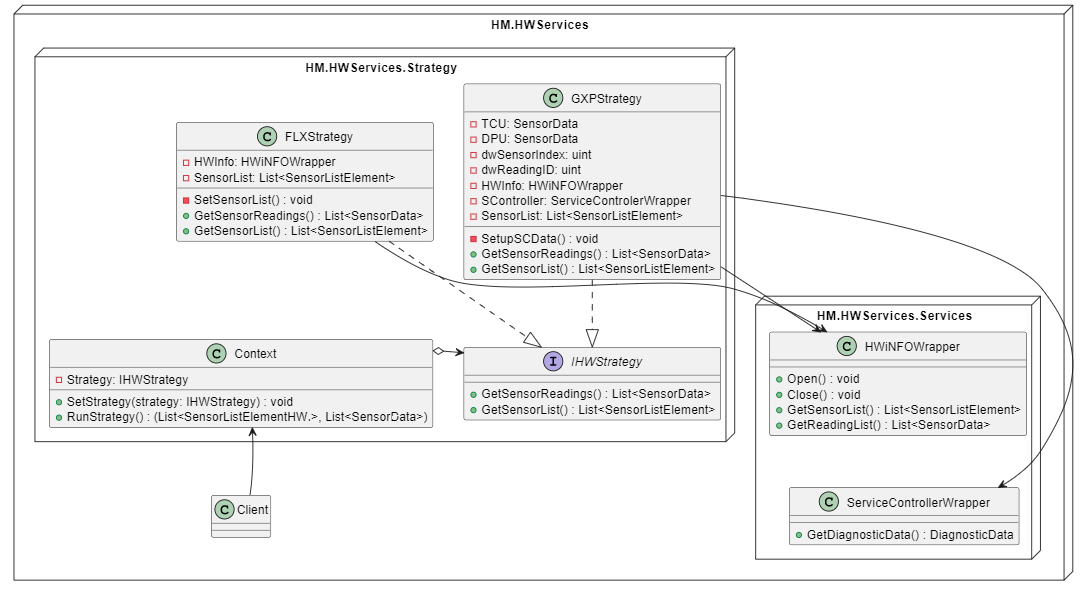
\includegraphics[width=1\textwidth]{UMLDatenerfassung.png}
        \caption{Architektur der HM.HWServices für das Auslesen der Hardware}
        \label{fig:HWServicesUML}
    \end{figure}
\end{center}
\vspace{-1.8cm}
Die Architektur der \textit{HM.HWServices} wird nach dem, in Abschnitt \ref{sec:StrategyPattern} beschrieben Strategie Muster ausgelegt.
Die Komponenten des Strategie Muster sind im Verzeichnis \textit{HM.HWServices.Strategy} organisiert.\\
Durch den \textit{Context} kann die gewünschte Strategie ausgewählt und aufgerufen werden. Die Client-Anwendung interagiert dabei ausschließlich mit dem \textit{Context}, der wiederum die gewünschten Funktionen der ausgewählten Strategieklasse aufruft.\\  
Da sich das Auswerten von VisuNet FLX und GXP voneinander unterscheidet, soll für jede Plattform eine eigene Strategieklasse verwendet werden. Jede dieser Strategieklassen wird hierbei von dem \textit{IHWStrategy} Interface abgeleitet. Dieses definiert die Struktur der Klassen, sodass die Funktionen der ausgewählten Klasse im \textit{Context} aufgerufen werden können, ohne die spezifische Strategieklasse genau zu kennen. Anschließend kann beim Start des Programms entschieden werden, welche dieser Strategien verwendet werden soll.\\
Muss das Programm in Zukunft um eine neue Hardwarekonfiguration einer Plattform erweitert werden, kann dies über das Hinzufügen einer weiteren Strategieklasse realisiert werden.\\
Zum Auslesen der Sensordaten stehen zunächst zwei Schnittstellen zur Verfügung. Die in Abschnitt \ref{sec:HWiNFO} beschriebene Shared Memory Funktion der \textit{HWiNFO} Software liefert die Messwerte der an das Mainboard angeschlossenen Sensoren. Die VisuNet FLX Plattform bedarf keiner weiteren Schnittstellen zum Lesen von Sensordaten.\\
Um die Temperatursensoren in \ac{dpu} und \ac{tcu} der VisuNet GXP Plattform auszulesen, wird eine weitere Bibliothek verwendet, welche die Kommunikation mit dem in der Plattform verbauten Servicecontroller ermöglicht.\\
Für beide Schnittstellen wurde jeweils eine Wrapperklasse (Siehe Abschnitt \ref{sec:AdapterPattern}) konzipiert, welche die wesentlichen Funktionen der Bibliotheken in einer übersichtlichen Klasse bereitstellen und die Datenstruktur der Schnittstelle adaptieren. Die Wrapperklassen werden im Verzeichnis \textit{HM.HWServices.Wrapper} organisiert. (Siehe Abbildung \ref{fig:HWServicesUML}).
\subsubsection*{Adaption der Schnittstelle}
Beim Auslesen der Sensorik über die \textit{HWiNFOWrapper} Klasse, können zwei Listen ausgelesen werden. Zum einen werden alle verfügbaren Sensoren der Plattform in einer Liste von \textit{SensorListElement} abgelegt. Zum anderen wird eine Liste des Typen \textit{SensorData} erzeugt. In dieser ist jeder Sensor mit dem aktuellen Messwertwert hinterlegt. Die Datentypen hierzu sind in Abbildung \ref{fig:DatastructuresUML} abgebildet.    
\begin{center}
    \begin{figure}[h!]
        \centering
        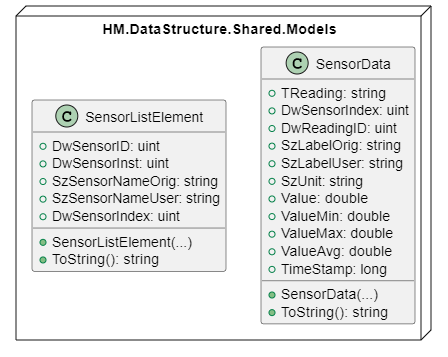
\includegraphics[width=0.45\textwidth]{UMLDatastructureHWI.png}
        \caption{Datenstruktur zum Zwischenspeichern der Sensordaten}
        \label{fig:DatastructuresUML}
    \end{figure}
\end{center}
\vspace{-1.8cm}

\subsubsection*{Strategie Konzept}
Ziel der Strategieklassen ist wie zuvor bereits erwähnt die Kapselung der Algorithmen zum Auslesen der Zielplattformsensorik. Eine Strategie soll daher folgende Daten zurückliefern: Zum einen soll eine Aufzählung aller Sensoren im System erstellt werden, und in einer Liste von \textit{SensorListElement} hinterlegt werden. (Siehe Tabelle \ref{fig:SensorList}) 
\vspace{-0.5cm}
\begin{center}
    \begin{table}[h!]
        \centering
        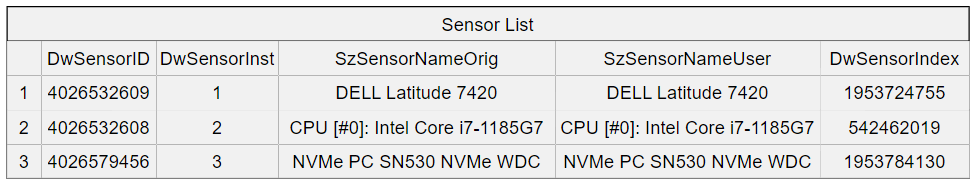
\includegraphics[width=0.7\textwidth]{SensorList.png}
        \caption{Beispiel einer Liste bestehend aus \textit{SensorListElement}}
        \label{fig:SensorList}
    \end{table}
\end{center}
\vspace{-1.8cm}
Zum anderen soll ein aktueller Auszug der Sensorwerte erstellt werden können. Hierzu sollen die Werte der einzelnen Sensoren in einer Liste von \textit{SensorData} gespeichert werden. (Siehe Tabelle \ref{fig:SensorReadings})
\vspace{-0.5cm}
\begin{center}
    \begin{table}[h!]
        \centering
        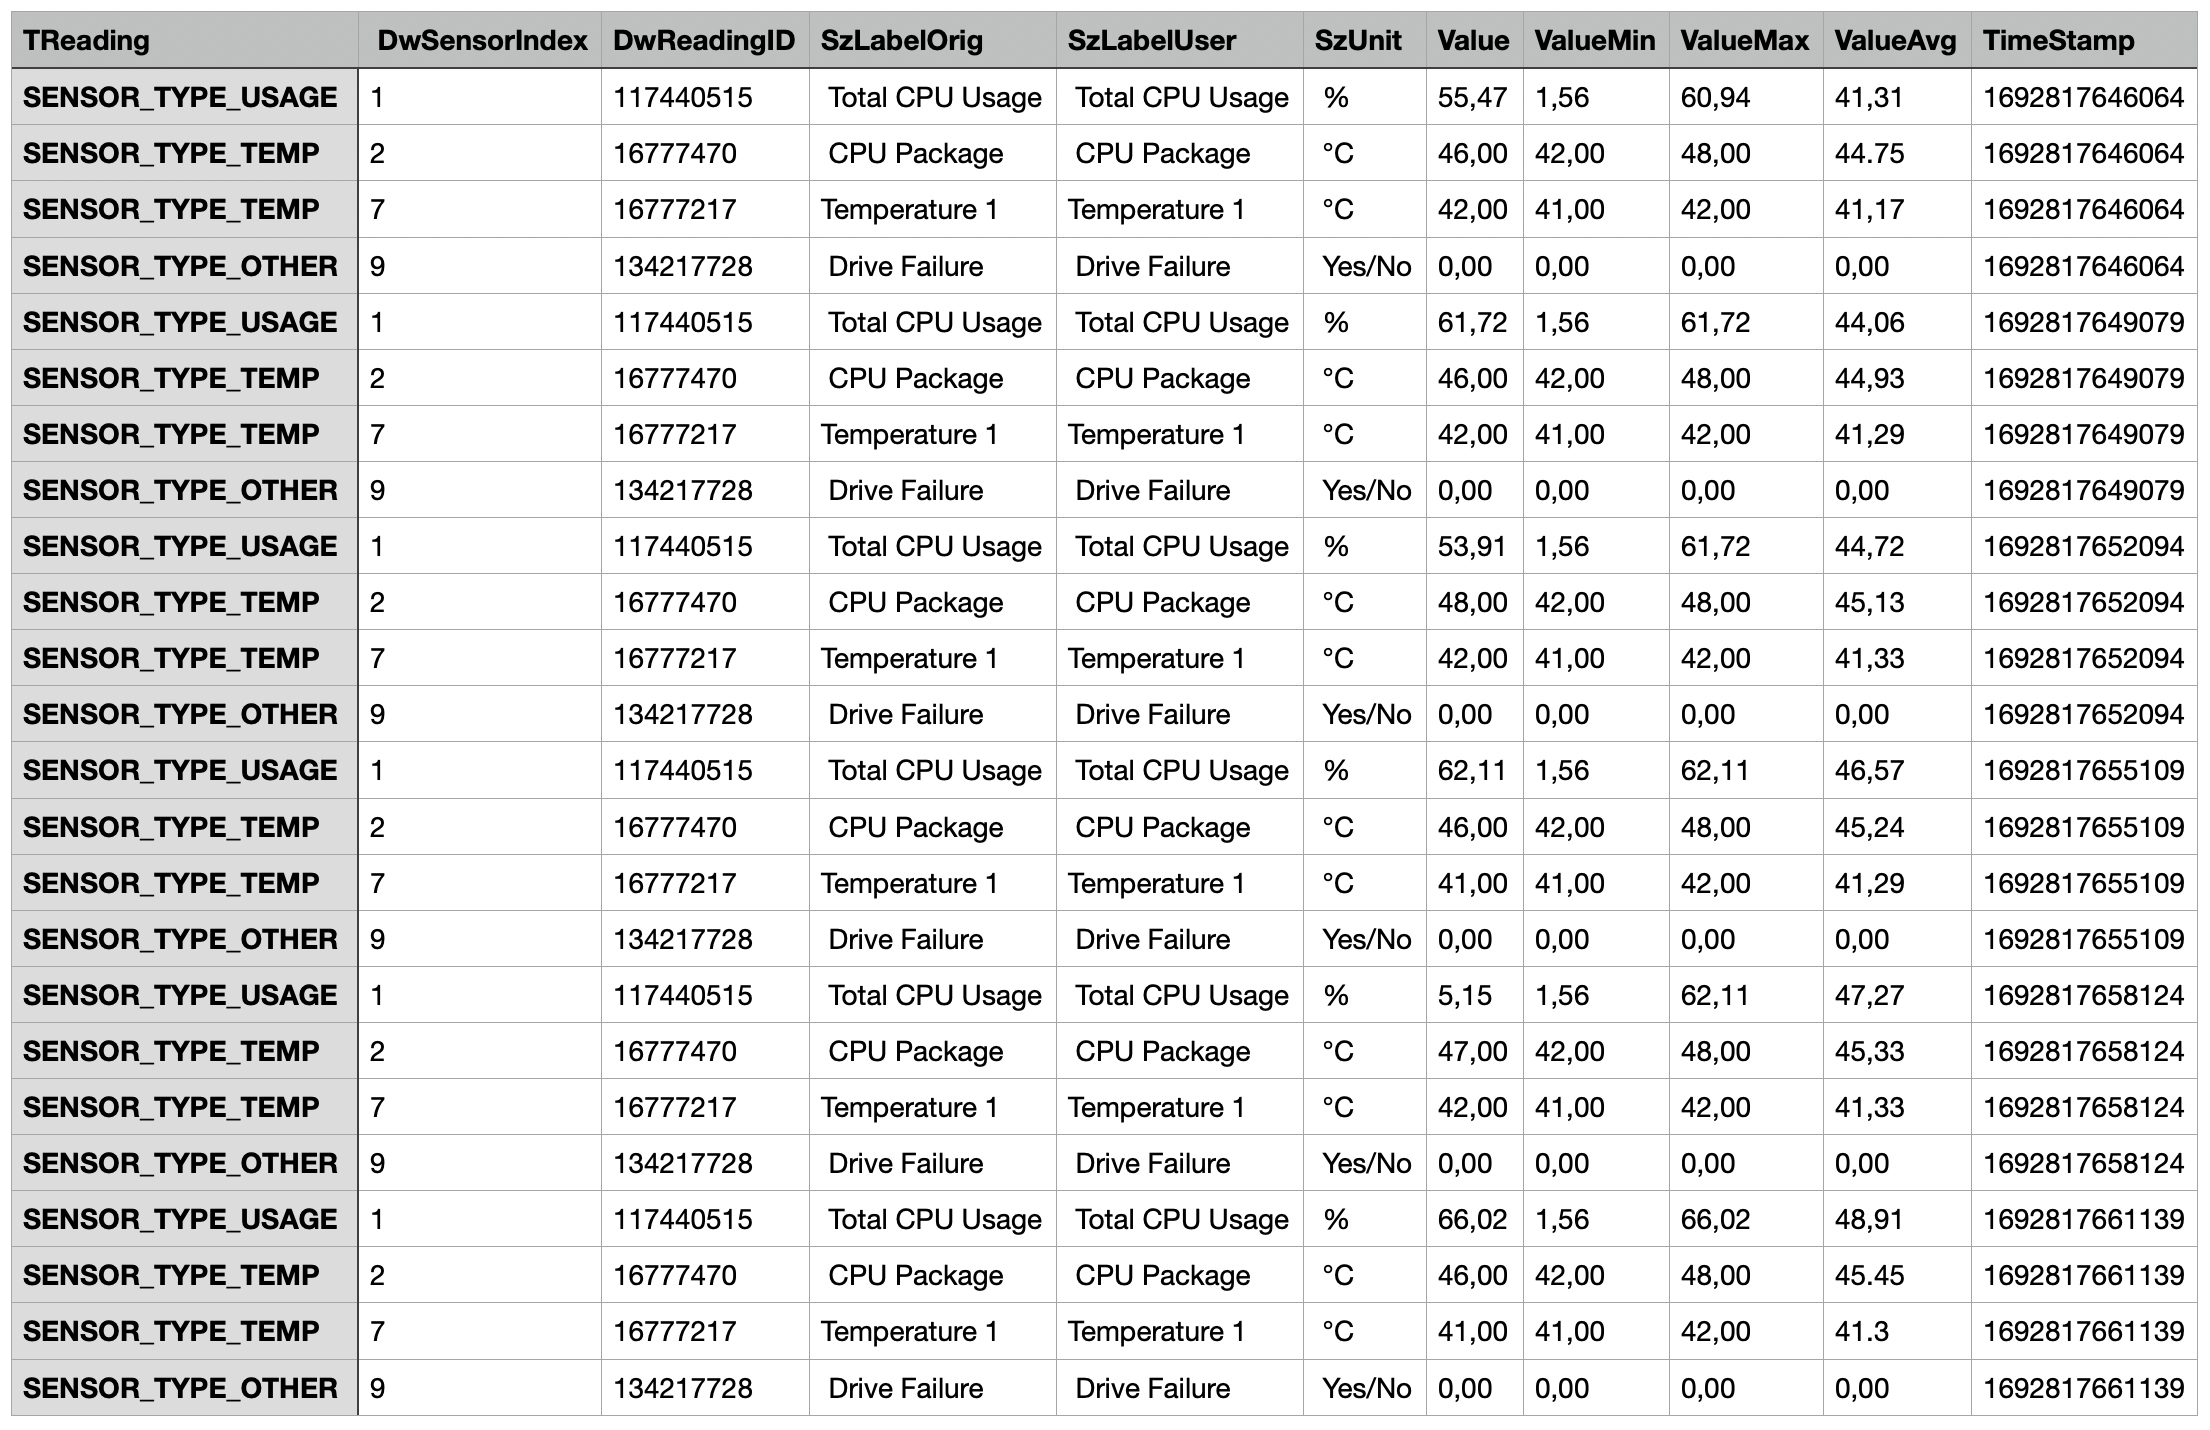
\includegraphics[width=0.81\textwidth]{SensorReadings.png}
        \caption{Beispiel einer Liste bestehend aus \textit{SensorData}}
        \label{fig:SensorReadings}
    \end{table}
\end{center}
\vspace{-1.8cm}
Da die \textit{HWiNFOWrapper} Schnittstelle alle verfügbaren Sensoren der VisuNet FLX Plattform abdeckt, ist die Strategie zum Auslesen dieser Plattform recht simpel. Dabei soll über einen Funktionsaufruf eine Liste mit den aktuellen Messwerten der Sensoren erstellt und zurückgegeben werden.\\
Der \textit{ServiceControllerWrapper} liefert, neben den Werten des \textit{HWiNFOWrapper}, \ac{dpu} und \ac{tcu} Temperaturen der VisuNet GXP Plattform. Die Datensätze der beiden Schnittstellen müssen daher in der \textit{GXPStrategy} kombiniert werden, sodass wie auch bei der \textit{FLXStrategy} jeweils eine Liste der Sensoren und eine Liste mit den Messwerten zurückgegeben wird (Siehe Tabelle \ref{fig:SensorList} und \ref{fig:SensorReadings}).\\
Mithilfe der Strategieklassen kann somit für jegliche Hardwarekonfiguration einer Plattform, eine gezielte Strategie erstellt werden, welche lediglich zwei Listen zurückliefert. Dabei ist der Anwendung selbst egal, welche und wie viel Schnittstellen verwendet werden.

\subsection{Entwurf eines Datenbankmodells zum Speichern der Messwerte}\label{sec:DatenbankModell}
Im vorherigen Abschnitt \ref{sec:AuslesenHardware} wurde eine Architektur zum Auslesen der plattformunabhängigen Sensoren beschrieben. Resultierend daraus steht dem Programm eine Schnittstelle bereit, welche eine Reihe von Messdaten zur Verfügung stellt. Ziel des Datenbankmodells ist es, die bereitgestellten Messdaten in einem strukturierten und übersichtlichen Format abzuspeichern.\\
\subsubsection*{Zuordnung der Datensätze}
Aus Tabelle \ref{fig:SensorReadings} geht hervor, dass die Datensätze der Tabelle grundsätzlich in drei Kategorien unterteilt werden können. Anhand der Spalte \textit{SzUnit} können die Daten in die Kategorien Temperatur (°C), Auslastung (\%) und Events (Yes/No) unterteilt werden. Bei weiterer Betrachtung der Datensätze wird zudem ersichtlich, dass sich die Einträge der Spalten \textit{TReading}, \textit{DwSensorIndex}, \textit{DwReadingID}, \textit{SzLabelOrig}, \textit{SzLabelUser} und \textit{SzUnit} bei jedem Sensor wiederholen.\\
Einhergehend aus dieser Beobachtung wurde die in Abbildung \ref{fig:DBModell} abgebildete Struktur der Datenbank erstellt. 
\begin{center}
    \begin{figure}[h!]
        \centering
        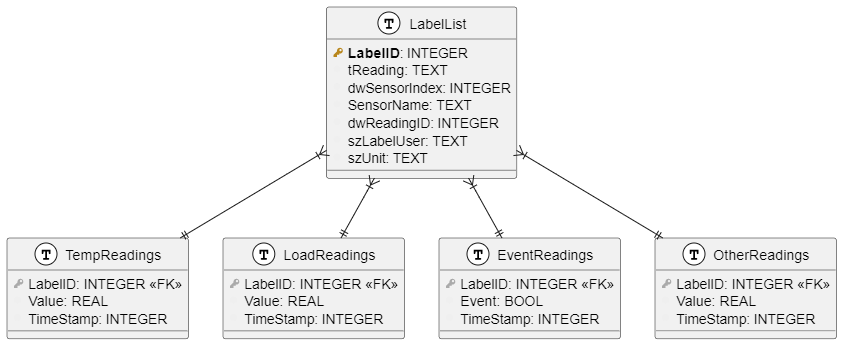
\includegraphics[width=1\textwidth]{DBModell.png}
        \caption{Datenbankmodell des Hardware-Health-Monitorings}
        \label{fig:DBModell}
    \end{figure}
\end{center}
\vspace{-1.8cm}
Die Datensätze der Tabellen \ref{fig:SensorList} und \ref{fig:SensorReadings} werden in fünf Datenbanktabellen unterteilt. Dabei werden die Felder \textit{TReading}, \textit{DwSensorIndex}, \textit{DwReadingID}, \textit{SzLabel} und \textit{SzUnit} in die Tabelle \textit{LabelList} ausgelagert. Hinzu kommt das Feld \textit{SensorName}, welches aus Tabelle \ref{fig:SensorList} stammt. Des Weiteren kommt das Feld \textit{LabelID} dazu, welches als Primärschlüssel konfiguriert wird. Über dieses Feld können nun die eigentlichen Messwerte aus den anderen Tabellen, den Sensoren zugeordnet werden. Die Messwerte werden dabei sortiert nach \textit{SzUnit} in vier Tabellen geschrieben. \textit{TempTabel} für Temperaturen in  °C, \textit{LoadReadings} für Auslastung in \%, \textit{EventTabel} für Events in 1/0 und \textit{OtherReadings} für alle andere Einheiten. Jede der vier Tabellen verfügt über ein Feld \textit{Value}, \textit{TimeStamp} und einem zugehörigen Schlüssel \textit{LabelID}.\\
Möchte man die Messwerte eines spezifischen Sensors erhalten, muss man zunächst den primär Schlüssel des Sensors aus der \textit{LabelList} Tabelle ermitteln. Über diesen erhält man anschließend die Werte des Sensors aus der entsprechenden Tabelle.
\subsubsection*{Erweiterung der Datenbank}
Zusätzlich zu den ausgelesenen Messwerten müssen auch die Ergebnisse der Systembewertung in der Datenbank abgelegt werden. 
Hierzu werden zunächst die Tabellen \textit{SystemStatus} und \textit{SystemMTBF} erstellt. Diese sind identisch und unterscheiden sich lediglich in der Bedeutung ihrer Werte. Der ermittelte Systemzustand wird in die Feldern \textit{Status}, \textit{Score} und \textit{Value} geschrieben. Die Felder \textit{TimeStampStart} und \textit{TimeStampEnd} grenzen das Intervall ein, in welchem der Systemzustand ermittelt wurde. Des Weiteren werden die Tabellen \textit{HistorySystemStatus} und \textit{SystemReliability} erzeugt. In diesen werden die historischen Werte des Systems, so wie dessen Verlässlichkeit gespeichert. (Siehe Abbildung \ref{fig:DBModellErweitert})   
\begin{center}
    \begin{figure}[h!]
        \centering
        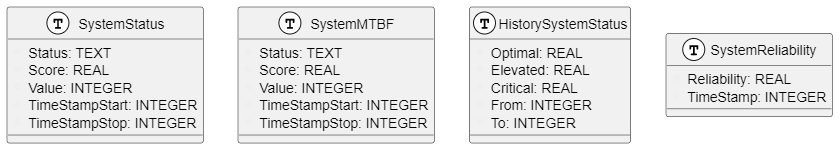
\includegraphics[width=1\textwidth]{DBErweitert.png}
        \caption{Datenbankmodellerweiterung des Hardware-Health-Monitorings}
        \label{fig:DBModellErweitert}
    \end{figure}
\end{center}
\vspace{-1.8cm}

\subsubsection*{Aufbau der Schnittstellen}
Um die komplexe Syntax der SQLite Engine zu kapsel, wird eine Wrapperklasse benötigt, welche die wesentlichen Datenbankaufrufe handhabt. Neben den Befehlen zum Erzeugen der Datenbank, bietet die \textit{SQLiteWrapper} Klasse auch die benötigten Funktionen um Datensätze von und in die Datenbank zu laden. Die Klasse wird im \textit{HM.DBServices} Verzeichnis organisiert. (Siehe Abbildung \ref{fig:HMDBServi}).
\vspace{-0.3cm}
\begin{center}
    \begin{figure}[h!]
        \centering
        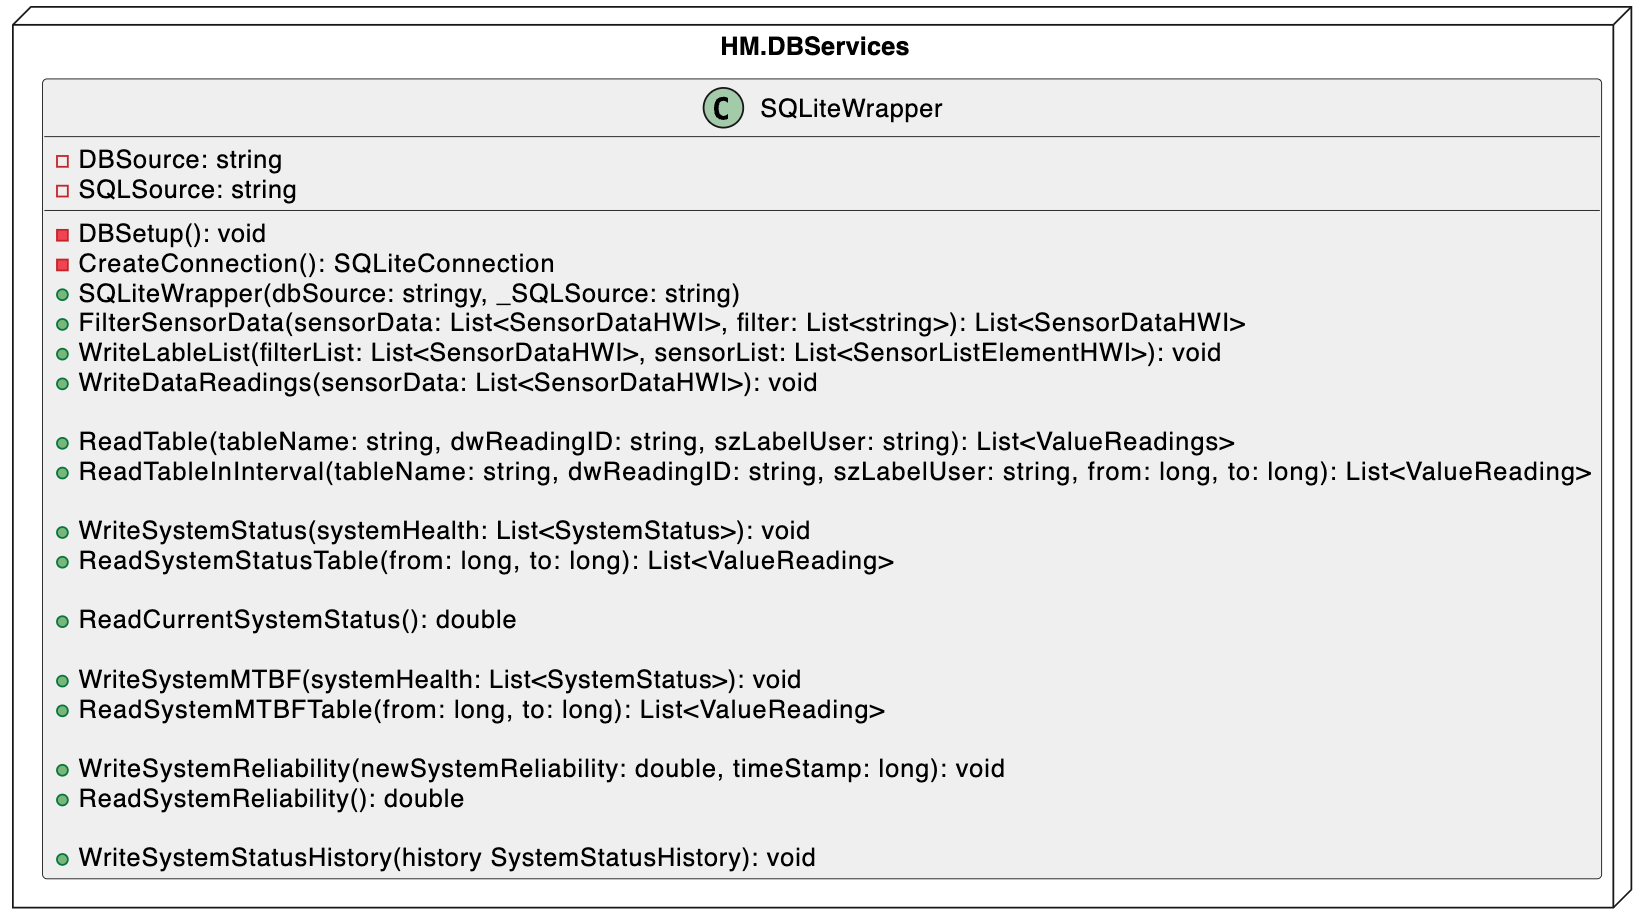
\includegraphics[width=1\textwidth]{HMDBService.png}
        \caption{Architektur des HM.DBService Verzeichnis}
        \label{fig:HMDBServi}
    \end{figure}
\end{center}
\vspace{-1.8cm}
Des Weiteren wird das \textit{HM.DataStrucutre.Shared.Models} Verzeichnis um die \textit{ValueReadings} Klasse erweitert. Diese besteht aus den Parametern \textit{Value} und \textit{TimeStamp}. Sie dient als Datentyp, über welchen einzelne Datensätze aus der Datenbank im Programm zwischengespeichert werden können. (Siehe Abbildung \ref{fig:ValueReadingsKlasse})
\begin{center}
    \begin{figure}[h!]
        \centering
        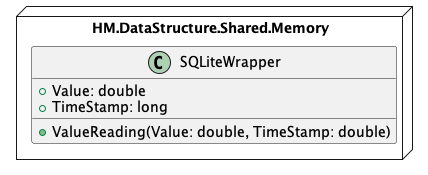
\includegraphics[width=0.5\textwidth]{HMDataStructure.png}
        \caption{Schnittstelle zum Auslesen einzelner Datensätze}
        \label{fig:ValueReadingsKlasse}
    \end{figure}
\end{center}





















